\section{Diseño}

\subsection{planteamiento de circuito}
Para este laboratorio se plantea el siguiente diagrama de conexiones hecho en el software \texttt{Proteus}.
\begin{figure}[h!]
    \centering
    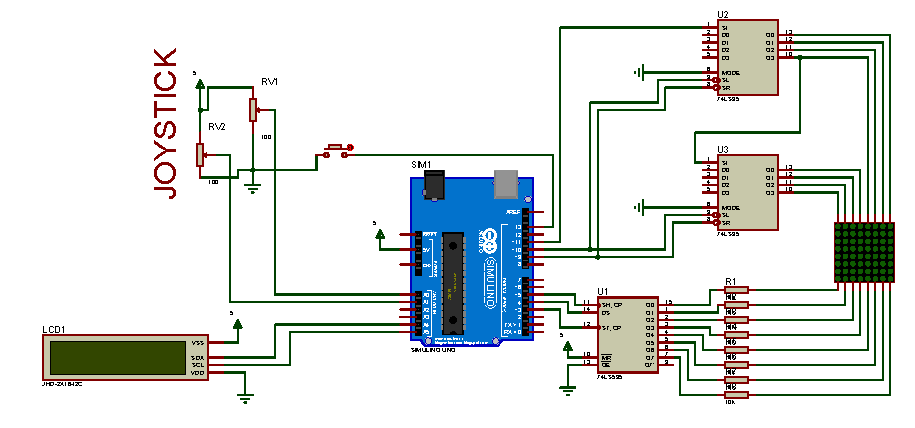
\includegraphics[width=0.9\textwidth]{Diagramas/xfcolor_cropped.pdf}
    \caption{Esquema de conexiones}
    \label{fig:esquema}
\end{figure}

Asi para el uso del registro de desplazamiento 74HC595 de 8 bits, se conectan 3 pines digitales hacia el integrado, siendo uno para enviar los datos en serie 
hacia el registro, otro para el reloj y el ultimo para el control del latch. La salida de este integrado se conecta a 8 resistencias de $\SI{220}{\ohm}$
para limitar la corriente de estos pines, finalmente este se conecta a la matriz LED 8x8. Tambien se utiliza el pin de alimentacion de $\$

Para los registros de desplazamiento de 4 bits, estos se tiene que conectar en cascada, para poder formar los 8 bits necesarios para controlar la matriz led.
Asi se utilizan 3 pines digitales para esta conexion
\subsection{Desarrollo del código}


